\documentclass{loyola-beamer}
\renewcommand{\titlelogo}{logo/luc-rev.svg}
\renewcommand{\slidelogo}{logo/luc.svg}
\usepackage{physics}
\usepackage{graphicx}
\usepackage{hyperref}

\renewcommand{\slidefoot}{Department of Physics -- PHYS422}
\def\c#1{\texttt{#1}}

\title{Manhattan Project}
\subtitle{A deep dive into the physics and history behind the atomic bombs project.}
\author{Ammar S. Alfaifi \& AbdulElah Hakami}
\date{\today}
\institute{NTiS}

\begin{document}

\begin{titleframe}{}
	\maketitle
\end{titleframe}

\begin{frame}{Contents}
	\tableofcontents
\end{frame}

\section{Origin}

\subsection{Mass–energy equivalence}

\begin{frame}
	\begin{figure}
		\begin{center}
			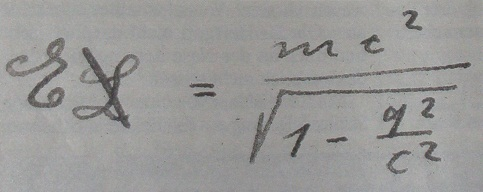
\includegraphics[width=0.7\textwidth]{./figures/E_mc_2.jpg}
		\end{center}
		\caption{The equation in Albert Einstein's own handwriting from 1912}\label{fig:e is mc2}
	\end{figure}
\end{frame}

\begin{frame}
	\begin{figure}
		\begin{center}
			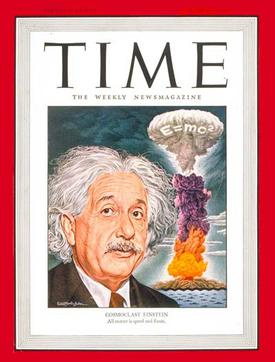
\includegraphics[height=0.5\textwidth]{./figures/Einstein_-_Time_Magazine.jpg}
		\end{center}
		\caption{The cover of Time magazine in July 1946.}\label{fig:The Time}
	\end{figure}
\end{frame}

\begin{frame}
	\begin{figure}
		\begin{center}
			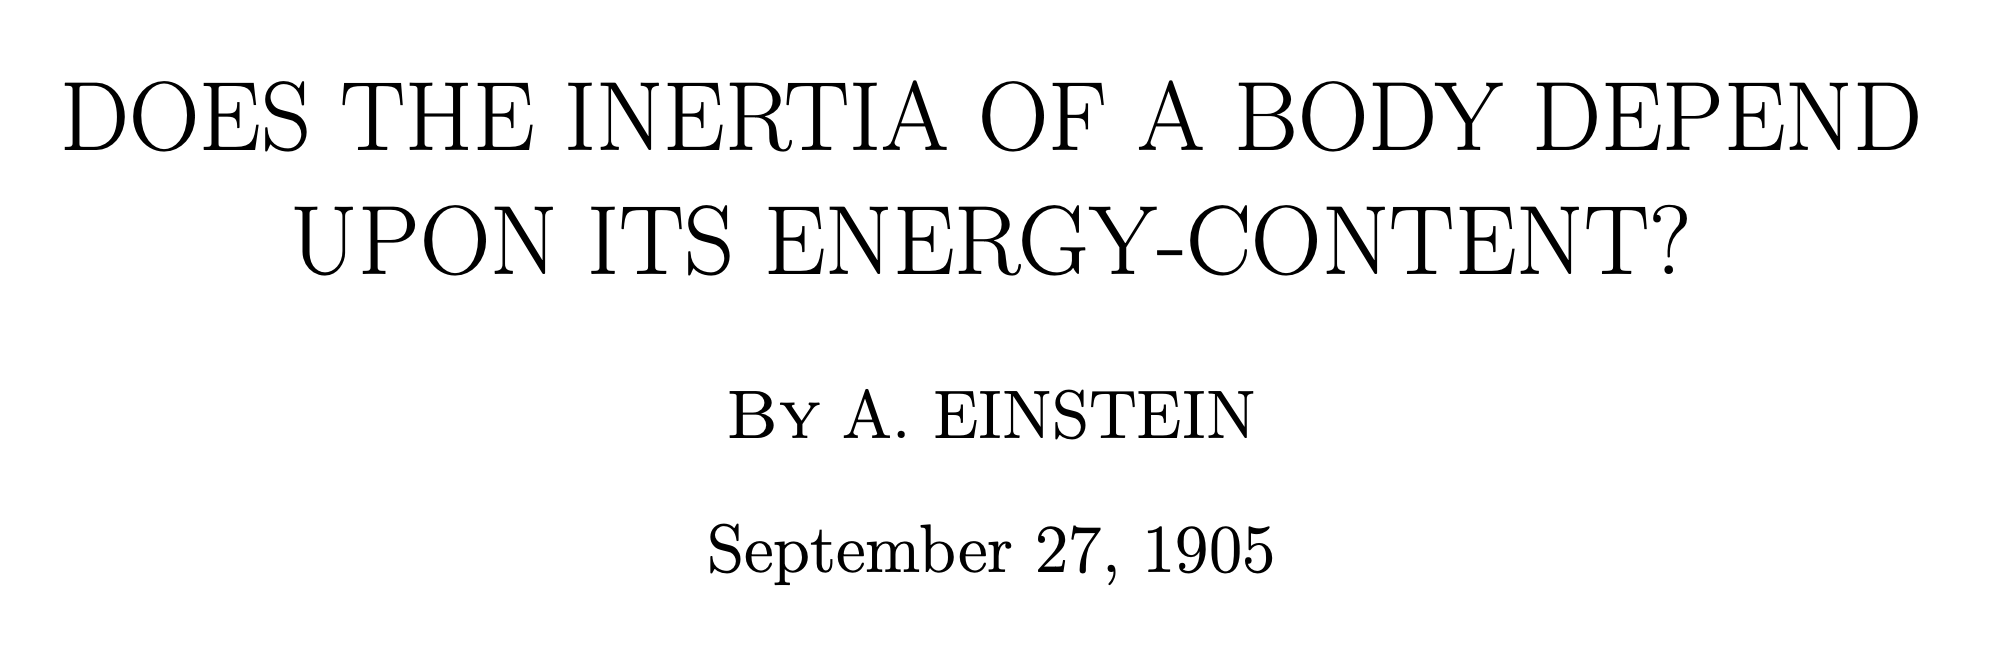
\includegraphics[width=0.9\textwidth]{./figures/einstein_paper.png}
		\end{center}
	\end{figure}
\end{frame}

\begin{frame}
	\begin{figure}
		\begin{center}
			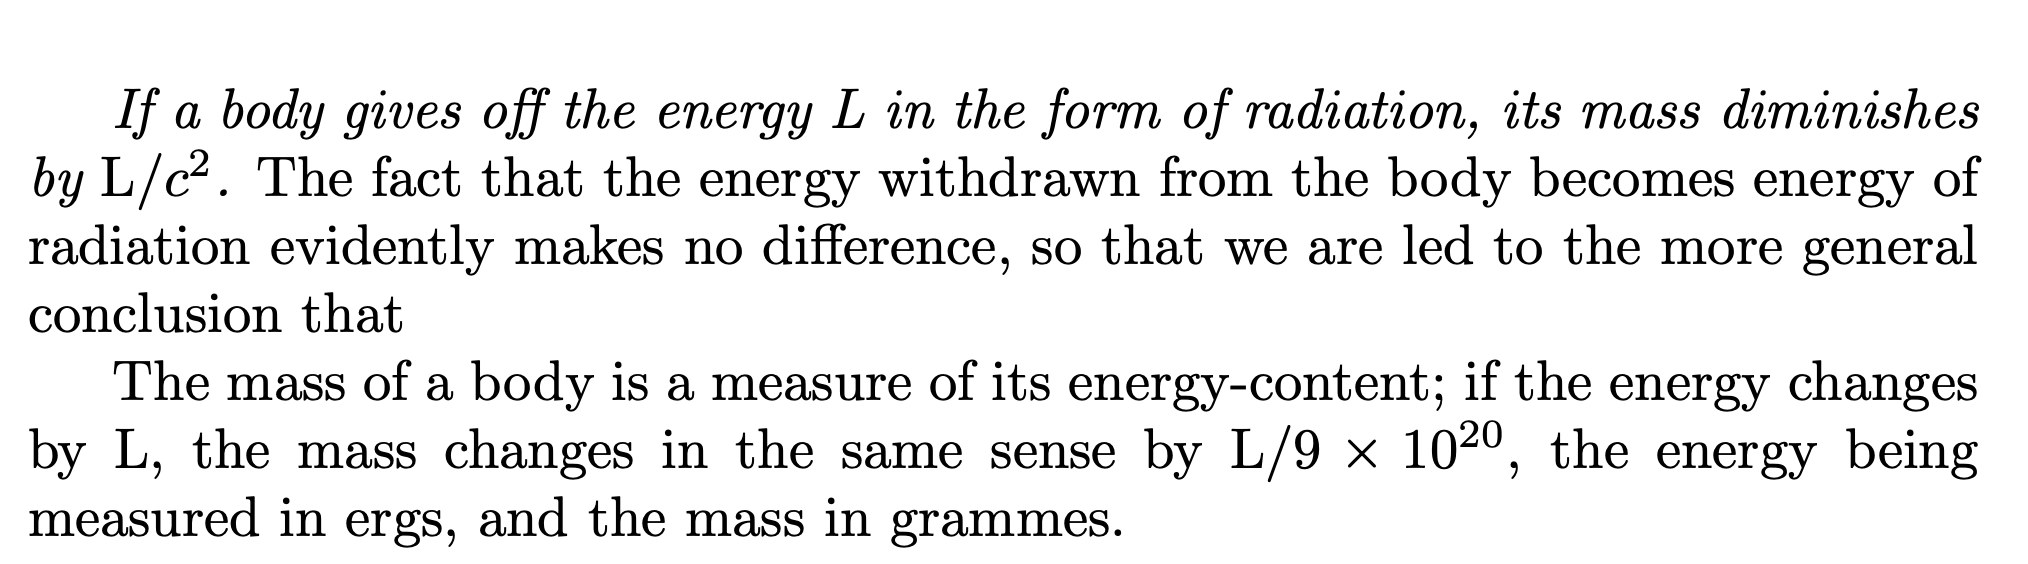
\includegraphics[width=0.9\textwidth]{./figures/einstein_paper_eq.png}
		\end{center}
	\end{figure}

	\begin{math}
		m = \frac{L}{c^2}
	\end{math}
	
\end{frame}

\begin{frame}
	\begin{center}
		\scalebox{5}{
			\begin{math}
				E = mc^2
			\end{math}
		}
	\end{center}
\end{frame}

\begin{frame}
	\begin{figure}
		\begin{center}
			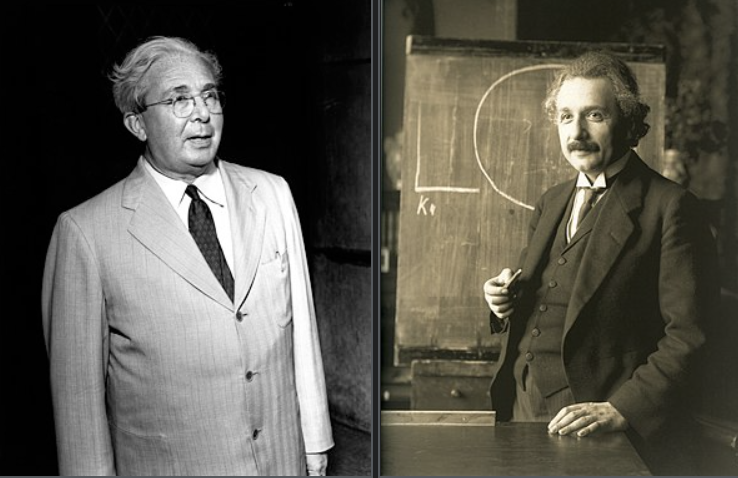
\includegraphics[width=0.7\textwidth]{./figures/leo-and-albert.png}
		\end{center}
		\caption{Leo Szilard and Albert Einstein.}\label{fig:leo and albert}
	\end{figure}
\end{frame}


\section{Manhattan Project}

% Start of the main contents
\begin{frame}{Introduction}
	\begin{itemize}
		\item In 1942, before the Manhattan Project, Robert Oppenheimer held conferences where physicists discussed nuclear bomb design issues.
		\item A gun-type design was initially chosen, where two sub-critical masses of plutonium would be brought together by firing a "bullet" into a "target".
		\item The alternative implosion-type design, suggested by Richard Tolman, was considered far more complex and received scant consideration.
	\end{itemize}
\end{frame}

\section{Thin Man}

\begin{frame}
	\begin{itemize}
		\item In early 1943, Oppenheimer prioritized the gun-type weapon but created the E-5 Group at Los Alamos to investigate implosion as a hedge against predetonation.
		\item Implosion-type bombs were determined to be more efficient in terms of explosive yield per unit mass of fissile material due to compressed fissile materials reacting more rapidly and completely.
		\item However, the plutonium gun-type bomb received the bulk of the research effort due to less uncertainty involved, with the assumption that the uranium gun-type bomb could be easily adapted from it.
	\end{itemize}
\end{frame}

\begin{frame}
	\begin{figure}
		\begin{center}
			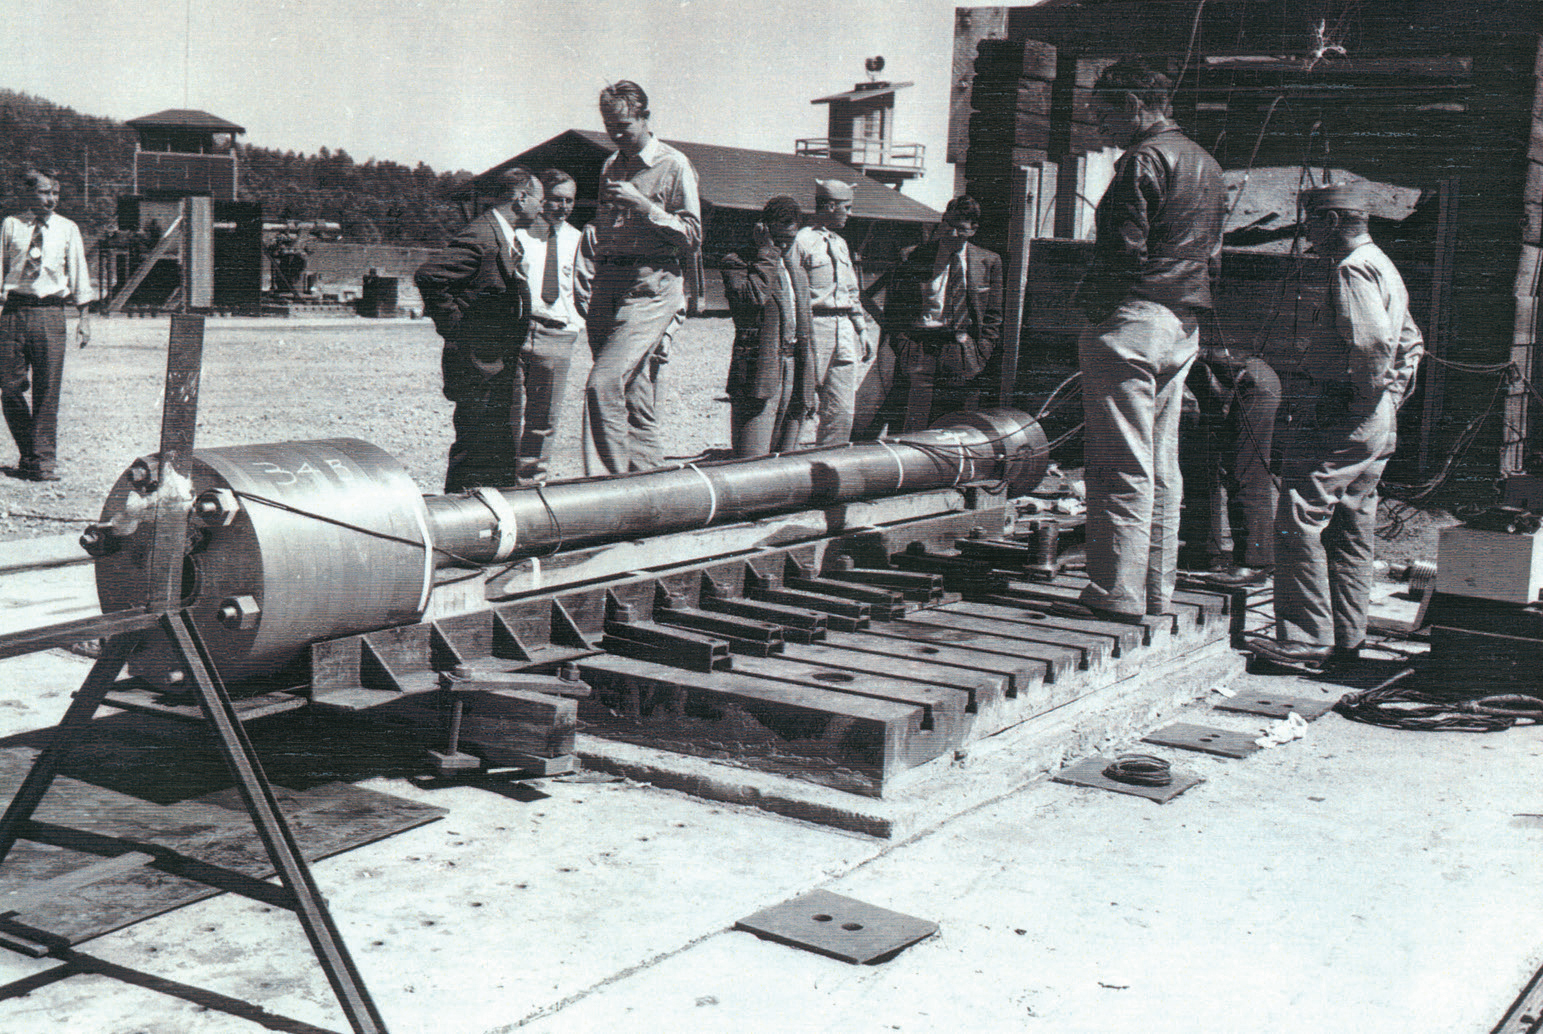
\includegraphics[width=0.7\textwidth]{./figures/Thin_Man_testing_at_Anchor_Ranch.jpg}
		\end{center}
		\caption{A prototype of the "Thin Man" gun being tested at Anchor Ranch, at Los Alamos.}\label{fig:thin man img}
	\end{figure}
\end{frame}

\begin{frame}
	\begin{itemize}
		\item "Thin Man" was an early nuclear weapon design proposed before plutonium breeding.
		\item It assumed plutonium could be assembled by a gun-type method, requiring a "bullet" speed of at least 910 m/s.
		\item Dimensions: 5.2 m long, 0.97 m wide tail and nose, 0.58 m midsection.
		\item Weight: approximately 3,600 kg.
		\item No USAAF aircraft could carry it without modifications.
		\item Avro Lancaster (10 m bomb bay) or modified Boeing B-29 Superfortress were suggested.
		\item B-29 modification involved removing part of the bulkhead and oxygen tanks (Serial No. 42-6259).
	\end{itemize}
\end{frame}

\begin{frame}
	\begin{figure}
		\begin{center}
			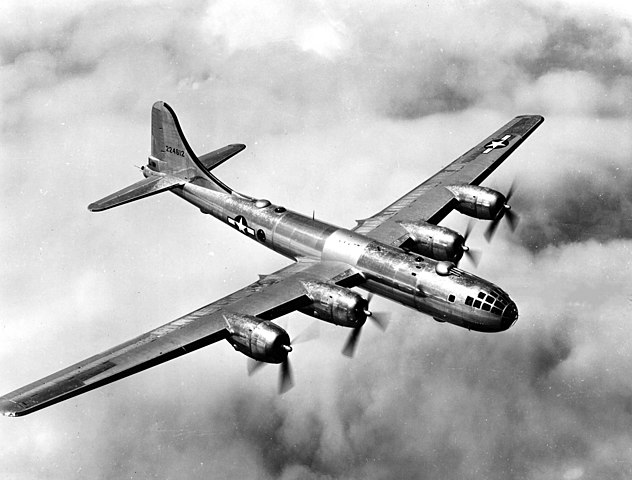
\includegraphics[width=0.6\textwidth]{figures/632px-B-29_in_flight.jpg}
		\end{center}
		\caption{A USAAF B-29 Superfortress. B-29s dropped the atomic bombs on Hiroshima and Nagasaki, the only aircraft ever to drop nuclear weapons in combat.}
	\end{figure}
\end{frame}

\subsection{Issues}

\begin{frame}{Predetonation}
	\begin{itemize}
		\item Experiments in April 1944 by Emilio G. Segrè's group at Los Alamos showed reactor-produced plutonium contained the isotope plutonium-240.
		\item Plutonium-240 has a high spontaneous fission rate, increasing the risk of predetonation.
		\item This meant the plutonium would likely predetonate and blow itself apart during critical mass formation.
		\item The distance required to avoid predetonation would need an impractically long gun barrel for any bomber.
	\end{itemize}
\end{frame}

\begin{frame}
	\begin{itemize}
		\item The only viable option was the more difficult implosion method.\cite{Hoddeson1993}
		\item At a meeting on July 17, 1944, it was agreed that gun-type work would focus on the \texttt{Little Boy} uranium design.
		\item Almost all Los Alamos research was re-oriented toward solving the implosion problems for the \texttt{Fat Man} plutonium bomb.
	\end{itemize}
\end{frame}

\begin{frame}
	\begin{figure}
		\includesvg[width=0.45\textwidth]{figures/Nuclear_predetonation.svg}
		\caption{If two pieces of subcritical material are not brought together fast enough, nuclear predetonation can occur, whereby a smaller explosion than expected will blow the bulk of the material apart.}
	\end{figure}
\end{frame}

\begin{frame}{Pu-239 Production}
	\begin{equation*}
		{ }_{92}^{238} \mathrm{U}+{ }_0^1 \mathrm{n} \longrightarrow{ }_{92}^{239} \mathrm{U} \xrightarrow[23.5 \text { min }]{\beta^{-}}{ }_{93}^{239} \mathrm{~Np} \xrightarrow[2.3565 \mathrm{~d}]{\beta^{-}}{ }_{94}^{239} \mathrm{Pu}
	\end{equation*}
	\vfill
	Neutrons from the fission of uranium-235 are captured by uranium-238 nuclei to form uranium-239; a beta decay converts a neutron into a proton to form neptunium-239 (half-life 2.36 days) and another beta decay forms plutonium-239.\cite{Greenwood1997}
\end{frame}

\begin{frame}
	\begin{tabular}{|l|l|l|l|}
		\hline
		Isotope                 & Decay mode                      & Half-life (years) & Spontaneous fission n (1/(g\cdot s)) \\
		\hline
		\textsuperscript{238}Pu & alpha to \textsuperscript{234}U & 87.74             & 2600                                 \\
		\hline
		\textsuperscript{239}Pu & alpha to \textsuperscript{235}U & 24100             & 0.022                                \\
		\hline
		\textsuperscript{240}Pu & alpha to \textsuperscript{236}U & 6560              & 910                                  \\
		\hline
	\end{tabular}
\end{frame}

\section{Little Boy}

\begin{frame}
	\begin{itemize}
		\item The gun-type uranium bomb, code-named "Little Boy", was much simpler than the plutonium implosion design.
		\item Its smaller size allowed it to fit into the B-29 bomb bay without difficulty.
		\item Design specifications were completed in February 1945, with components manufactured at different plants.
		\item The bomb (except uranium payload) was ready by early May 1945.
		\item The enriched uranium projectile and target were completed in June and July 1945, respectively.
		\item No full test of the gun-type bomb was conducted before the Hiroshima bombing.
	\end{itemize}
\end{frame}

\begin{frame}
	\begin{figure}
		\begin{center}
			\includesvg[width=0.6\textwidth]{figures/Gun-type_fission_weapon_en-labels_thin_lines.svg}
		\end{center}
		\caption{The "gun" assembly method. When the hollow uranium projectile was driven onto the target cylinder, a nuclear explosion resulted.}
	\end{figure}
\end{frame}

\begin{frame}
	\begin{itemize}
		\item Little Boy had an estimated yield of 15 kilotons based on data from instruments dropped by parachute.
		\item A rule of thumb was developed: the "5 psi lethal area" where overpressure $\geq$ 34 kPa would be fatal.
		\item At Hiroshima, this lethal area had a diameter of 3.5 km.
		\item Three main effects: blast, fire, and radiation.
	\end{itemize}
\end{frame}

\begin{frame}{Blast}
	\begin{itemize}
		\item Everything within 1 km was destroyed except reinforced concrete buildings.
		\item Severe blast damage followed the 34 kPa overpressure contour at 1.8 km radius.
		\item Fuel for fires was created by blast damage to structures.
	\end{itemize}
\end{frame}

\begin{frame}{Fire}
	\begin{itemize}
		\item Fireball surface temperature was $6,000^\circ$C, igniting fires across the destruction zone.
		\item Fires merged into a 3.2 km diameter firestorm within 20 minutes.
		\item An estimated 60\% of immediate deaths were from fires.
	\end{itemize}
\end{frame}

\begin{frame}{Radiation}
	\begin{itemize}
		\item No local fallout since it was an air burst.
		\item Lethal radius of 1.3 km from initial radiation.
		\item 30\% of immediate deaths from direct radiation exposure.
		\item 30\% of survivors had radiation injuries, increasing cancer risk.
	\end{itemize}
\end{frame}

\subsection{The Disaster}

\begin{frame}
	\begin{figure}
		\begin{center}
			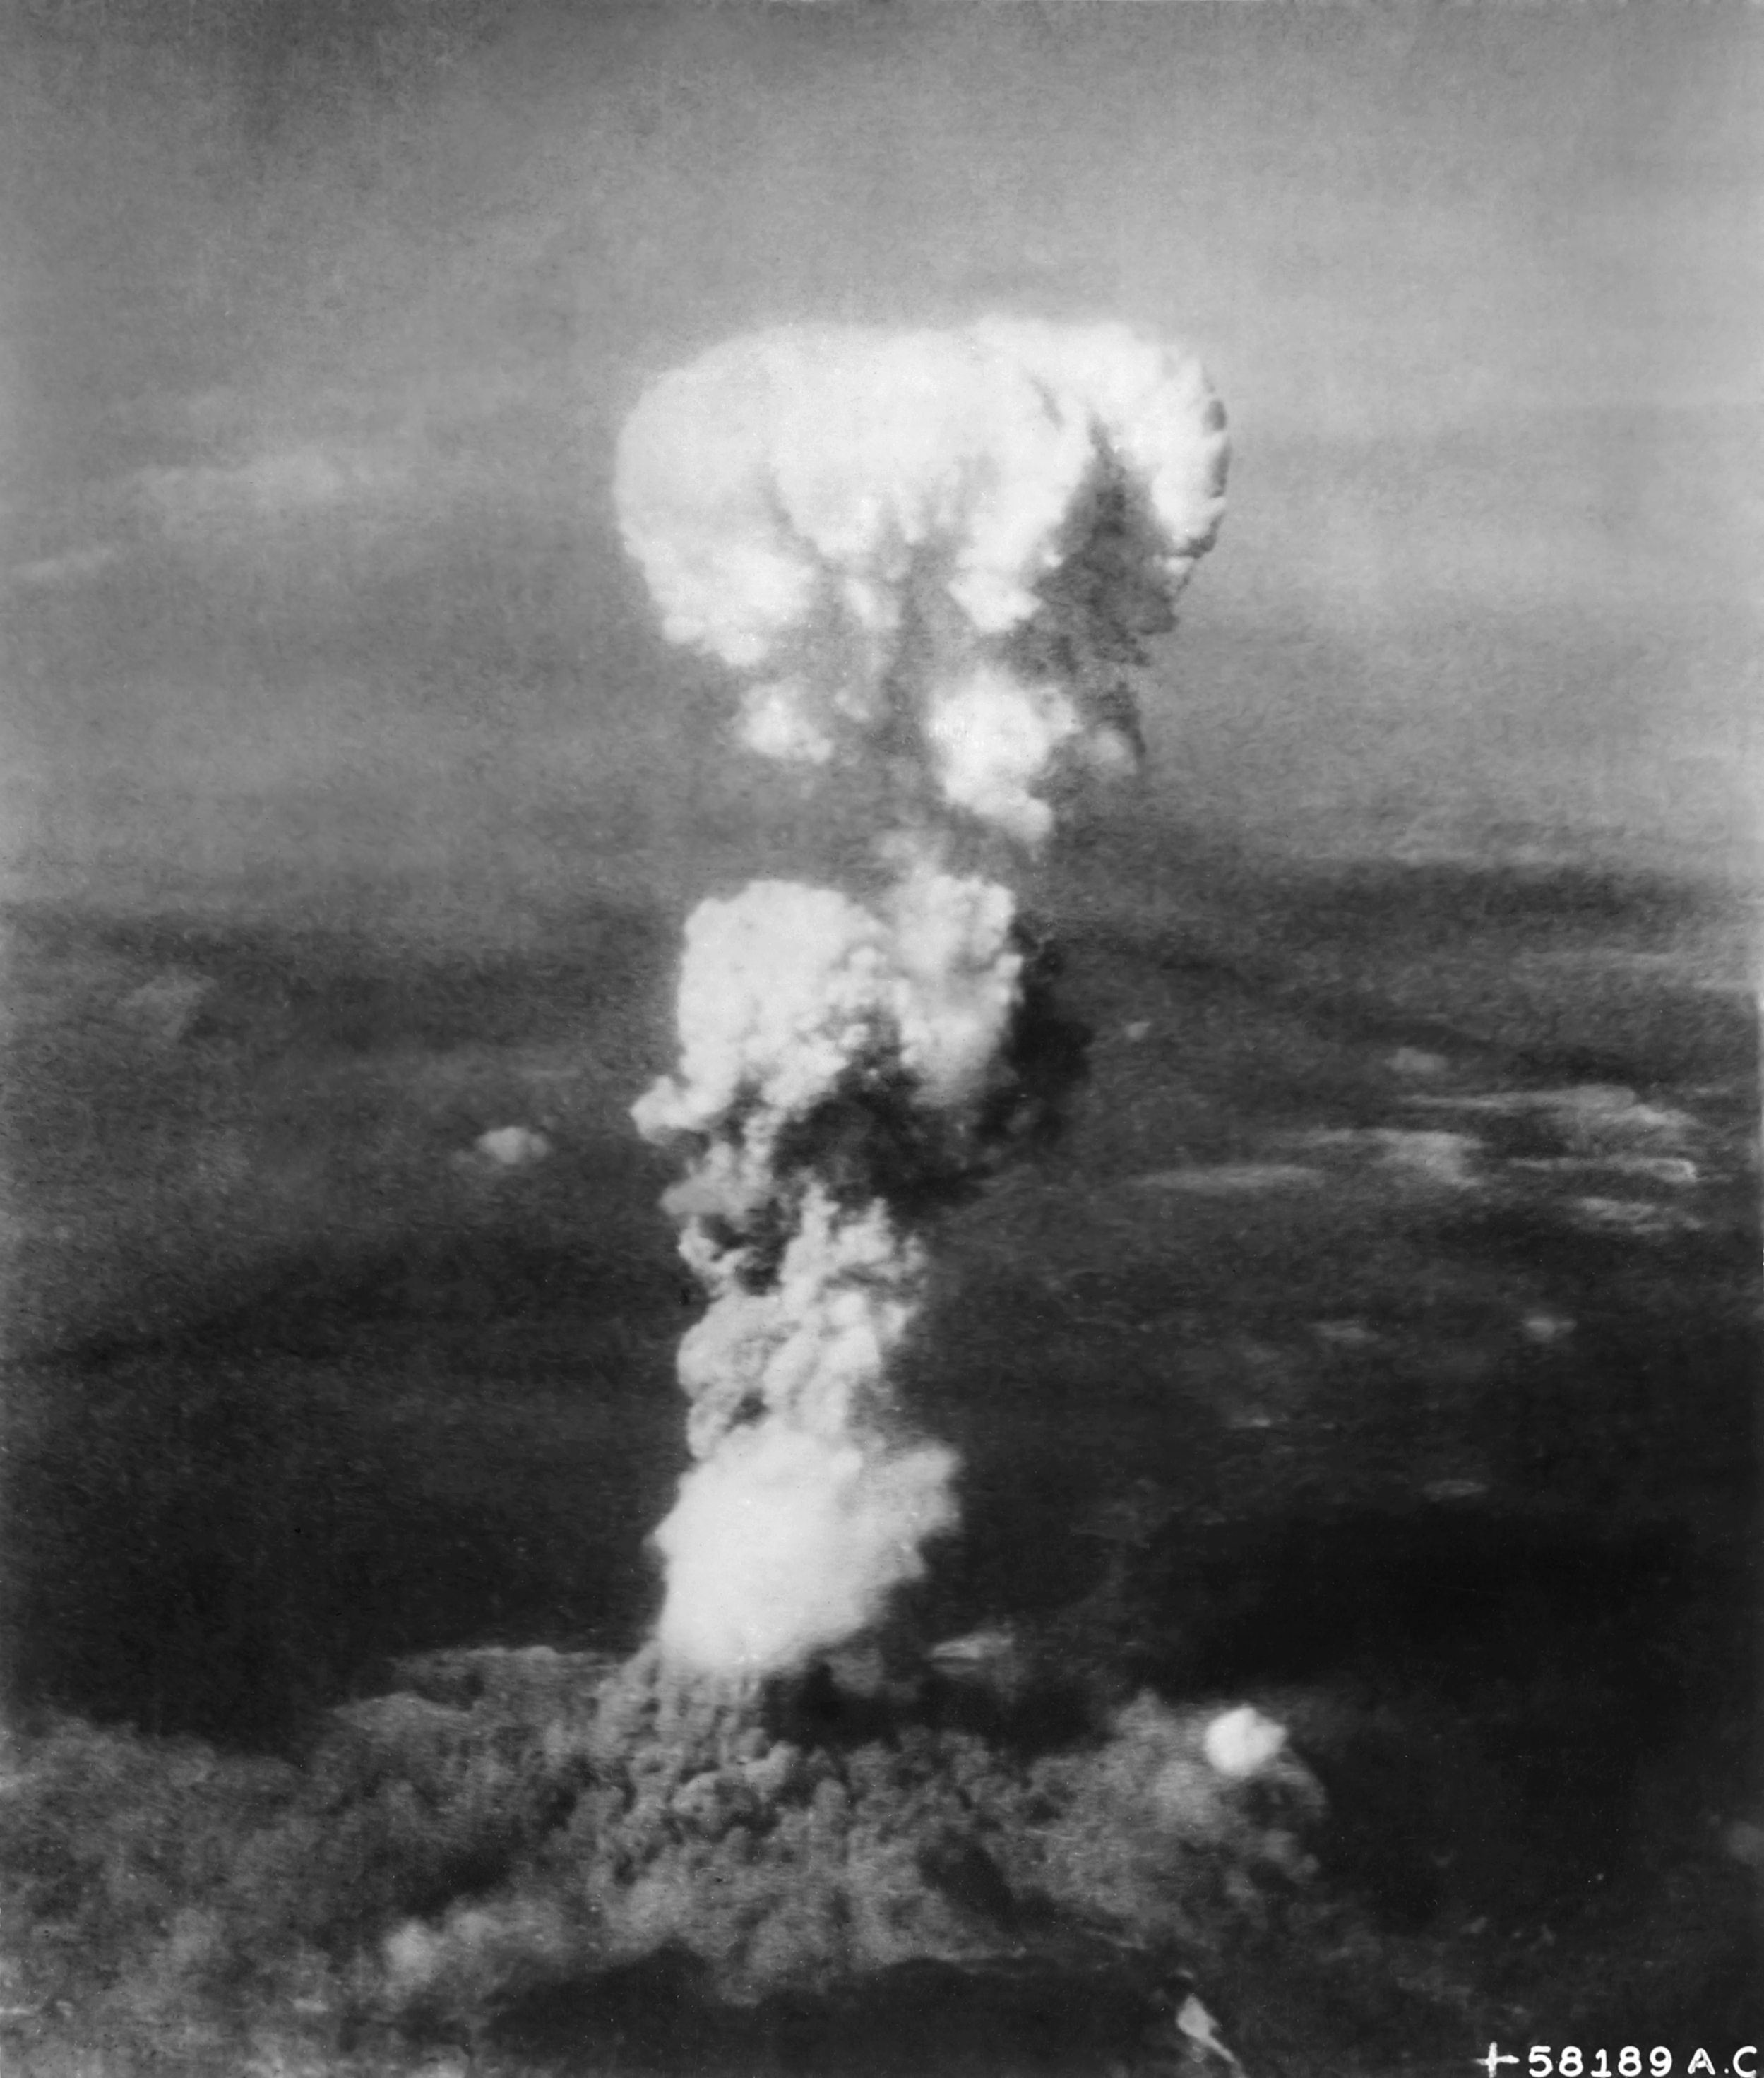
\includegraphics[width=0.4\textwidth]{figures/Atomic_cloud_over_Hiroshima_-_NARA_542192_-_Edit.jpg}
		\end{center}
		\caption{The mushroom cloud over Hiroshima after the detonation of Little Boy on 6 August 1945.}
	\end{figure}
\end{frame}

\begin{frame}
	\begin{itemize}
		\item After falling for 44.4 seconds. Detonation occurred at an altitude of 600 $\pm$ 15 m.
		\item It was less powerful than the Fat Man bomb dropped on Nagasaki.
		\item However, damage and casualties in Hiroshima were higher due to its flat terrain.
		\item Published figures in 1945 stated 66,000 people killed and 69,000 injured.
		\item Later estimates put the death toll as high as 140,000.
	\end{itemize}
\end{frame}

\begin{frame}
	\begin{figure}
		\begin{center}
			\includegraphics[width=0.6\textwidth]{figures/Spare_Little_Boy_atomic_bomb_casing_at_the_Imperial_War_Museum_in_London_in_November_2015.jpg}
		\end{center}
		\caption{One of five casings built for the Little Boy bomb used on Hiroshima on display at the Imperial War Museum in London during 2015}
	\end{figure}
\end{frame}

\section{Fat Man}

\begin{frame}
	\begin{itemize}
		\item The idea of using shaped charges as 3D explosive lenses came from James L. Tuck and was developed by John von Neumann.
		\item Precision in the inward motion of the explosive plates was crucial, achieved using exploding-bridgewire detonators invented by Luis Alvarez and Lawrence Johnston.
		\item Robert Christy's calculations showed that a solid plutonium sphere could be compressed to a critical state, simplifying the task.
		\item The bomb size was constrained by the available aircraft; (maximum length: 3.4 m, width: 1.5 m, weight: 9,100 kg).
		\item Drop tests led to modifications, including the addition of a "California Parachute" stabilizer for a stable descent.
		\item The final wartime Y-1561 design was assembled with 90 bolts and yielded approximately 100 TJ (25 kilotonnes) in the Trinity test on July 16, 1945.
	\end{itemize}
\end{frame}


\begin{frame}
	\begin{figure}
		\begin{center}
			\includesvg[width=0.7\textwidth]{figures/Fat_Man_External.svg}
		\end{center}
		\caption{Fat Man external schematic. }
	\end{figure}
\end{frame}

\begin{frame}
	\begin{figure}
		\begin{center}
			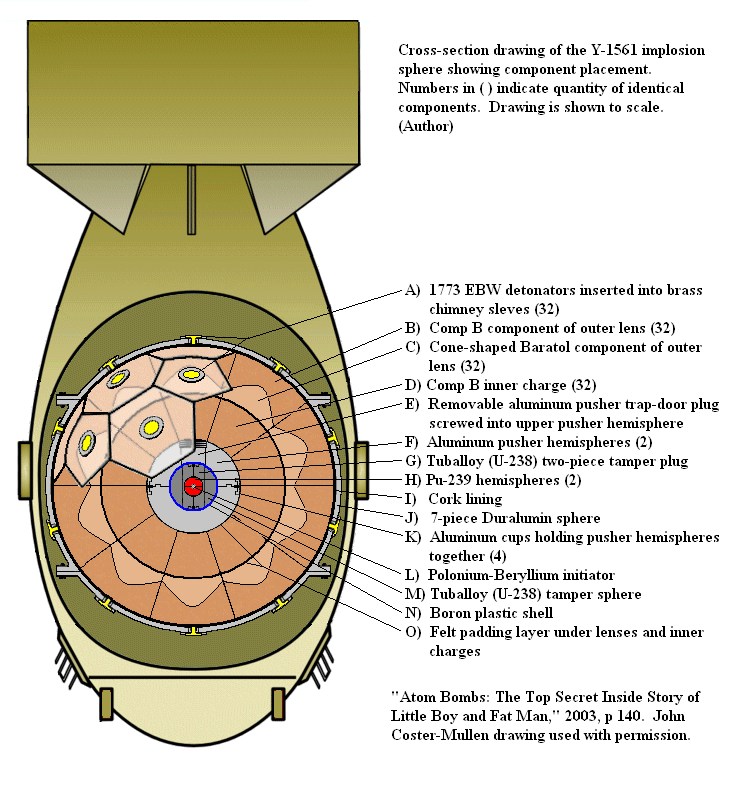
\includegraphics[width=0.5\textwidth]{figures/Fat_Man_Internal_Components.png}
		\end{center}
		\caption{Fat Man internal schematic}
	\end{figure}
\end{frame}

\begin{frame}{The Implosion}
	\url{https://upload.wikimedia.org/wikipedia/commons/0/05/ImplosionShapedCharge.gif}
\end{frame}

\begin{frame}{The Urchin}
	\begin{itemize}
		\item The neutron initiator design typically combines beryllium-9 and polonium-210, separated until activation.
		\item The alpha source isotope must have strong alpha emissions and weak gamma emissions.
		\item It consisted of a beryllium pellet (0.8 cm diameter), beryllium shell (2 cm outer diameter, 0.6 cm wall thickness) with grooves, and polonium-210 (50 curies, 11 mg) deposited between them.
	\end{itemize}
\end{frame}

\begin{frame}
	\begin{itemize}
		\item Gold and nickel coatings shielded the beryllium from polonium's alpha particles.
		\item Upon implosion, the shock wave mixed the beryllium and polonium, allowing alpha particles to bombard beryllium and emit neutrons (1 neutron every 5-10 ns).
		\item The neutrons triggered the chain reaction in the compressed plutonium core.
	\end{itemize}
\end{frame}

\begin{frame}
	\url{https://youtube.com/clip/UgkxPCbwqQO4_6HBbKd4qxSKm2mrt0CYYnDy?si=m5m0Mrrw2ZoW0jmk}
\end{frame}

\begin{frame}
	\begin{figure}
		\begin{center}
			\includegraphics[width=0.4\textwidth]{figures/Nagasakibomb.jpg}
		\end{center}
		\caption{Mushroom cloud after Fat Man exploded over Nagasaki on 9 August 1945}
	\end{figure}

\end{frame}

\section{References \& Conclusion}

% --- Conclusion --- %

% --- References --- %
\begin{frame}{References}
	\bibliographystyle{plain}
	\bibliography{references}
\end{frame}

% ---- The End ---- %
\begin{titleframe}{Thank you for listening.}
\end{titleframe}

\end{document}
